\documentclass[12pt]{article}
% \usepackage[margin=1.25in]{geometry}
\usepackage[inner=2.0cm,outer=2.0cm,top=2.5cm,bottom=2.5cm]{geometry}
\usepackage{color}
\usepackage{graphicx}
\usepackage{amssymb}
\usepackage{amsmath}
\usepackage{amsthm}
\usepackage{bm}
\usepackage{hyperref}
\usepackage{multirow}
\usepackage{mathtools}
\usepackage{enumerate}


\newcommand{\homework}[5]{
	\pagestyle{myheadings}
	\thispagestyle{plain}
	\newpage
	\setcounter{page}{1}
	\noindent
	\begin{center}
		\framebox{
			\vbox{\vspace{2mm}
				\hbox to 6.28in { {\bf KRP \hfill #2} }
				\vspace{6mm}
				\hbox to 6.28in { {\Large \hfill #1 \hfill} }
				\vspace{6mm}
				\hbox to 6.28in { {\it Instructor: {\rm #3} \hfill Name: {\rm #4}, StudentId: {\rm #5}}}
				\vspace{2mm}}
		}
	\end{center}
	% \markboth{#4 -- #1}{#4 -- #1}
	\vspace*{4mm}
}


\begin{document}
\large
	%==========================Put your name and id here==========================
	\homework{Homework 1}{Spring 2023}{YiZheng Zhao}{张运吉}{211300063}
    \paragraph{Question 1. Basic Understanding of KR and Ontologies}~{}
    \\
    
    A Logic-based ontology is a formal, explicit specification of a shared conceptualization and has decidability and rationality.
For areas of interest based on a fixed vocabulary, knowledge can be expressed in terms of finite
words and then determined and reasoned by the formal logic syntax.For example, we can use syllogism to
reason more knowledge. \par
    If we interpret domains and concepts as sets and elements of sets,the
KR model can be calculated semantically using set theory. We can also interpret some logical words as sets
operations, such as unions, intersections, and subsets, are also computational.

    \paragraph{Question 2. Expressivity \& Computability}~{}
    \\

	Example: Has Mary eaten yet? \par
    My opinion: Expressiveness and computability are trade-offs.The more expressive a logic-based KR language is, the weaker it may be in some ways,
    such as completeness, soundness and decidability. For example, FOL is more expressive than ALC, but FOL is undecided and decidabile while ALC is 
    decidabile and computabile.More than that, Natural language is as expressive as
    possible in any circumstances, but it is not a computational model. Therefore, a logic-based KR language is not more expressive, more suitable for knowledge representation, but also to examine its computability.

    \paragraph{Question 3. Manchester Syntax}~{}
    \\

    \begin{enumerate}
        \item[(1)]
            Timo is a cow.
        \item[(2)]
            No.
        \item[(3)] 
            Not enough.
        \item[(4)]
            zero.
    \end{enumerate}

    \paragraph{Question 4. ALC Extensions \& FOL}~{}
    \\

    \begin{enumerate}
        \item[(1)]
        \begin{enumerate}
            \item[(1.1)]
            Sentence: Every Chinese couple has at most 3 children. \\
            Concept names: ChineseCouple \\
            Role names: hasChildren \\
            Inclusion: ChineseCouple $\sqsubseteq$ ($\leq$ 3 hasChildren.$\top$) \\
            \item[(1.2)]
            Sentence: ML is a course taught by SFM who is a professor working at NJU. \\
            Concept names: Course, Professor \\
            Role names: taughtBy, workingAt \\
            Nominals: ML, SFM, NJU \\
            Inclusion: $\{ \text{ML} \} \sqsubseteq \text{ Course } \sqcap (\exists \text{taughtBy}.\{ \text{SFM} \})$ \\
            $\{ \text{SFM} \} \sqsubseteq \text{ Professor } \sqcap (\exists \text{ workingAt}.\{ \text{NJU} \})$ \\
            \item[(1.3)]
            Sentence: NJU is a university whose members are a school or a department. \\
            Concept names: University, School, Department \\
            Role names: hasMember \\
            Nominals: NJU \\ 
            Inclusion: $\{ \text{NJU} \} \sqsubseteq \text{University } \sqcap (\exists \text{ hasMember}.\top) \sqcap (\forall \text{ hasMember}.(\text{School}\sqcup \text{Department}))$ \\
            \item[(1.4)]
            Sentence:  NJU has at least 30,000 students. \\
            Concept names: Students \\
            Role names: has \\
            Nominals: NJU \\
            Inclusion: $\{ \text{NJU} \} \sqsubseteq (\ge 30,000 \text{ has}.\text{Student})$ \\
            \item[(1.5)]
            Sentence:  All members of AI School are undergraduates, graduates, or teachers. \\
            Concept names: Undergraduates, Graduates, Teacher \\
            Role names: memberOf \\
            Nominals: AI school \\
            Inclusion: $\forall \text{ memberOf}.\{ \text{AI school} \} \sqsubseteq \text{Undergraduate} \sqcup \text{Graduate} \sqcup \text{Teacher}$
            \item[(1.6)]
            Sentence:  The domain of the relation “citizenOf” consists of countries. \\
            Concept names: Country \\
            Role names: citizenOf \\
            Inclusion: $\exists \text{ citizenOf}^{-}.\top \sqsubseteq \text{Country}$ \\
        \end{enumerate}
        \item[(2)] 
        \begin{enumerate}
            \item[(2.1)]
            $\forall x(\text{memberOf}(x, \text{AI School}) \to \text{Undergraduate}(x) \lor \text{Graduate}(x) \lor \text{Teacher}(x))$
            \item[(2.2)] 
            $\forall x(\exists y(\text{citizenOf}(y, x)) \to \text{Country}(x))$
        \end{enumerate}
    \end{enumerate}

    \paragraph{Question 5. DL Semantics}~{}
    \\

    \begin{enumerate}
        \item[(1)]
        True. We only need one example to prove it. \\
        Ontology: $\top \sqsubseteq \bot$, with no empty domain $\Delta^{\mathcal{I}}$.
        \item[(2)]
        False. \\
        If there is an ontology has finite models, we can always replace an element in the domain with a new element (which is not in the original domain), so we get a new model.
        Because the new elements are infinite, we can construct an infinite number of models.
        \item[(3)] 
        True. \\
        Based on the results of the previous two questions, obviously every ontology has either no model or infinite many models.
        \item[(4)]  
        True. \\
        According to the def of satisfiability, a class C is satisfiable w.r.t $\mathcal{T}$ iff
        $C^{I} \neq \emptyset$ for some model $\mathcal{I}$ of $\mathcal{T}$. \\
        $\because C^{I} \neq \emptyset \therefore \mathcal{I}$ is a non-empty interpretation of C.
        \item[(5)]
        False. \\
        If there is an unsatisfied class in a model with a non-empty interpretation, then it also satisfies the definition
        of satisfiable class that conflicts with the original statement.
        \item[(6)]
        True. \\
        According to the result of (5),   we know that an unsatisfiable class is interpreted as an empty set($C^{I} = \emptyset$), so it will be a subclass of any other class.
    \end{enumerate}

    \paragraph{Question 6. Interpretation as Graph}~{}
    \\

    \begin{enumerate}
        \item[(1)]
        $(\lnot A)^{\mathcal{I}} = \{ f, h, i \}$
        \item[(2)] 
        $(\exists r.(A \sqcup B))^{\mathcal{I}} = \{ d, f \}$
        \item[(3)] 
        $(\exists s.\exists s.\lnot A)^{\mathcal{I}} = \{ d, e \}$
        \item[(4)] 
        $(\lnot A \sqcap \lnot B)^{\mathcal{I}} = \{ f, h, i \}$
        \item[(5)]
        $(\forall r.(A \sqcup B))^{\mathcal{I}} = \{ d, f, g, h, i \}$
        \item[(6)]
        $(\le 1s.\top)^{\mathcal{I}} = \{ e, f, g, h, i \}$
    \end{enumerate}

    \paragraph{Question 7. DL Semantics}~{}
    \\

    \begin{enumerate}
        \item[(1)]
        $(Q \sqcap {\ge 2r.P})^{\mathcal{I}} = \emptyset$ \\
        $(\forall r.Q)^{\mathcal{I}} = \{ b, c, d, e \}$ \\
        $(\lnot \exists r.Q)^{\mathcal{I}} = \{ b, c, e \}$ \\
        $(\forall r.\top \sqcap \exists r^{-}.P)^{\mathcal{I}} = \{ b, d, e \}$ \\
        $(\exists r^{-}.\bot)^{\mathcal{I}} = \emptyset$
        \item[(2)]
        \begin{enumerate}
            \item[(2.1)] 
            $(A \sqcap B)^{\mathcal{I}} = \emptyset$ \\
            $(\exists r.B)^{\mathcal{I}} = \{ 1, 2 \}$ \\
            $(\exists r.(A \sqcap B))^{\mathcal{I}} = \emptyset$ \\
            $\top^{\mathcal{I}} = \{ 1, 2, 3, 4, 5, 6 \}$ \\
            $(A \sqcap \exists r.B)^{\mathcal{I}} = \{ 1, 2 \}$ \\
            \item[(2.2)]
            $\mathcal{I} \models A \equiv \exists r.B$ \\
            $\mathcal{I} \models A \cap B \sqsubseteq \top$ \\
            $\mathcal{I} \models \exists r.A \sqsubseteq A \sqcap B$ \\
        \end{enumerate}
    \end{enumerate}

    \paragraph{Question 8. DL Semantics}~{}
    \\

    \begin{enumerate}
        \item[(1)]
        True. \\
        $\because C \sqsubseteq D \therefore C^{\mathcal{I}} \subseteq D^{\mathcal{I}}$for all models of $C \sqsubseteq D$ \\
        which means: $\forall x \in \Delta^{\mathcal{I}}, \text{if x} \in  C^{\mathcal{I}}, \text{then x}  \in  D^{\mathcal{I}}$ \\
        $
        \begin{aligned}
        (\exists r.C)^{\mathcal{I}} &= \{ x \in \Delta^{\mathcal{I}} | \exists y \in  \Delta^{\mathcal{I}} \mathrm{ s.t. } (x, y) \in r^{\mathcal{I}} \text{ and } y \in C^{\mathcal{I}} \} \\
        &\subseteq \{ x \in \Delta^{\mathcal{I}} | \exists y \in  \Delta^{\mathcal{I}} \mathrm{ s.t. } (x, y) \in r^{\mathcal{I}} \text{ and } y \in D^{\mathcal{I}} \} \\
        &= (\exists r.D)^{\mathcal{I}}
        \end{aligned}
        $ \\
        $\therefore \exists r.C \sqsubseteq \exists r.D$ holds.(completeness of DL)
        \item[(2)]
        False. \\
        A counterexample: \\
        $\Delta^{\mathcal{I}} = \{a, b, c\}$ \\
        $C^{\mathcal{I}} = \{c\}$ \\
        $r^{\mathcal{I}} = \{(a, a), (b, b)\}$ \\
        $\therefore (\exists r.C)^{\mathcal{I}} = \emptyset,  \le 1r.\top = \{ a, b \}$ \\
        $(\exists r.C)^{\mathcal{I}} \neq (\le 1r.\top)^{\mathcal{I}}$ \\
        $\therefore \exists r.C$ is not equivalent to $\le 1r.\top$(completeness of DL)
        \item[(3)]
        True. \\
        For any models $\mathcal{I}$, \\
        \begin{equation}
            \begin{aligned}
                (\le 0r.\top)^{\mathcal{I}} &= \{ x \in \Delta^{\mathcal{I}} | \text{card}\left( \{ y \in \Delta^{\mathcal{I}} | (x, y) \in r^{\mathcal{I}} \text{ and } y \in \top^{\mathcal{I}} \} \right) \le 0  \} \\
                &= \{ x \in \Delta^{\mathcal{I}} | \{ y \in \Delta^{\mathcal{I}} | (x, y) \in r^{\mathcal{I}} \text{ and } y \in \Delta^{\mathcal{I}} \} = \emptyset  \} \\
                &= \{ x \in \Delta^{\mathcal{I}} | \{ y \in \Delta^{\mathcal{I}} | (x, y) \in r^{\mathcal{I}} \} = \emptyset  \} \\
            \end{aligned} 
        \end{equation}
        \begin{equation}
            \begin{aligned}
                (\forall r.\bot)^{\mathcal{I}} &= \{ x \in \Delta^{\mathcal{I}} | \forall y \in \Delta^{\mathcal{I}} \text{ if } (x, y) \in r^{\mathcal{I}} \text{ then } y \in \bot^{\mathcal{I}} \} \\
                &= \{ x \in \Delta^{\mathcal{I}} | \forall y \in \Delta^{\mathcal{I}} \text{ if } (x, y) \in r^{\mathcal{I}} \text{ then } y \in \emptyset \} \\
                &= \{ x \in \Delta^{\mathcal{I}} | \{ y \in \Delta^{\mathcal{I}} | (x, y) \in r^{\mathcal{I}} \} = \emptyset  \} \\
            \end{aligned} 
        \end{equation}
        $\therefore (\le 0r.\top)^{\mathcal{I}} = (\forall r.\bot)^{\mathcal{I}}$ \\
        Because of completeness of DL, we can know that$\le 0r.\top$ is equivalent to $\forall r.\bot$
        \item[(4)]
        False. \\
        A counterexample: \\
        $\Delta^{\mathcal{I}} = \{a, b, c\}$ \\
        $A^{\mathcal{I}} = \{a, c\}$ \\
        $B^{\mathcal{I}} = \{b\}$ \\
        $r^{\mathcal{I}} = \{(a, b), (a, c)\}$ \\
        $\therefore (\forall r.(A \sqcup B))^{\mathcal{I}} = \{ a, b, c \},  ((\forall r.A) \sqcup (\forall r.B))^{\mathcal{I}} = \{ b, c \}$ \\
        $(\forall r.(A \sqcup B))^{\mathcal{I}} \neq ((\forall r.A) \sqcup (\forall r.B))^{\mathcal{I}}$ \\
        $\therefore \forall r.(A \sqcup B)$ is not equivalent to $(\forall r.A) \sqcup (\forall r.B)$.(completeness of DL)
        \item[(5)]
        True. \\
        "$\Longrightarrow$": \\
        $\forall a \in \left(\exists r.(A \sqcup B)\right)^{\mathcal{I}}, \exists (a, b) \in r^{\mathcal{I}} \text{ and } (b\in A^{\mathcal{I}} \text{ or } b \in B^{\mathcal{I}})$ \\
        $\therefore a\in ((\exists r.A) \sqcup (\exists r.B))^{\mathcal{I}}$ \\
        "$\Longleftarrow$": \\
        $\forall c \in ((\exists r.A) \sqcup (\exists r.B))^{\mathcal{I}}, \exists d \in A^{\mathcal{I}} \text{ or } B^{\mathcal{I}} \text{ s.t. } (c, d) \in r^{\mathcal{I}}$ \\
        $\therefore c \in \left(\exists r.(A \sqcup B)\right)^{\mathcal{I}}$ \\
        $\therefore \left(\exists r.(A \sqcup B)\right)^{\mathcal{I}} = \left((\exists r.A) \sqcup (\exists r.B)\right)^{\mathcal{I}}$ \\
        $\therefore \exists r.(A \sqcup B)$is equivalent to $(\exists r.A) \sqcup (\exists r.B)$.(completeness of DL)
    \end{enumerate}

    \paragraph{Question 9. DL Semantics}~{}
    \\

    $\Delta^{\mathcal{I}} = \{a, b, c\}$ \par
    $Person^{\mathcal{I}} = \{a, b, c\}$ \par
    $Parent^{\mathcal{I}} = \{a, b\}$ \par
    $Mother^{\mathcal{I}} = \{a\}$ \par
    $hasChildren^{\mathcal{I}} = \{(a, c), (b, c)\}$ \par
    $\therefore \mathcal{I} \models \mathcal{T}, \mathcal{I} \not \models \text{Parent} \sqsubseteq \text{Mother}$.

    \paragraph{Question 10. DL Semantics}~{}
    \\

    \begin{enumerate}
        \item[(1)]
        $\Longrightarrow$:\\
        According to the def of subsumption, $X \sqsubseteq _{\mathcal{T}} Y$ iff $X^{\mathcal{I}} \subseteq Y^{\mathcal{I}}$ for all models $\mathcal{I}$ of $\mathcal{T}$. \\
        $\therefore  X^{\mathcal{I}} \cap \lnot Y^{\mathcal{I}} = \emptyset$ for all models $\mathcal{I}$ of $\mathcal{T}$. \\
        $\therefore X \sqcap \lnot Y$ is not satisfibale with respect to $\mathcal{T}$. \\
        $\Longleftarrow$:\\
        if $X \sqcap \lnot Y$ is not satisfibale with respect to $\mathcal{T}$, then for all models $\mathcal{I}$ of $\mathcal{T}$, we have $(X \sqcap \lnot Y)^{\mathcal{I}} = \emptyset$ \\
        $\therefore X^{\mathcal{I}} \cap \lnot Y^{\mathcal{I}} = \emptyset$ for all models $\mathcal{I}$ of $\mathcal{T}$ \\
        $X^{\mathcal{I}} \subseteq Y^{\mathcal{I}}$for all models $\mathcal{I}$ of $\mathcal{T}$ \\
        According to the def of subsumption, $X \sqsubseteq _{\mathcal{T}} Y$.
    \item[(2)]
        According to the result of (1), let $Y = \bot$, we have $X \sqsubseteq _{\mathcal{T}}\bot$ iff $X \sqcap \lnot \bot = X$ is not satisfibale with respect to $\mathcal{T}$. \\
        The inverse negation of the above inference is the conclusion we want to prove: $X$ is satisfiable with respect to $\mathcal{T}$ iff $X \not \sqsubseteq \bot$. \\

    \end{enumerate}

    \paragraph{Question 11. Bisimulation invariance}~{}
    \\

    \newpage
    \begin{enumerate}
        \item[(1)]
        \begin{figure}[h]
			\centering
			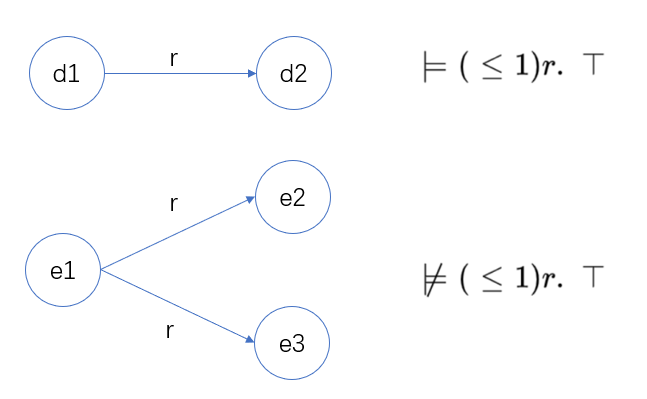
\includegraphics[width=0.8\textwidth]{11_1.png}\\
			\label{fig:roc}
			\end{figure}
        As shown in the picture above, $(\mathcal{I}_1, d_1) \sim (\mathcal{I}_2, e_1)$, so there is not a \\
        ALC-Concept could distinguish $d_1$ and $e_1$, but ALCQ-Concept $(\leq 1)r. \top$ can distinguish $d_1$ and $e_1$. \\
        Therefore $\mathcal{ALCQ}$ is more expressive than $\mathcal{ALC}$.
    \newpage
        \item[(2)]
        \begin{figure}[h]
			\centering
			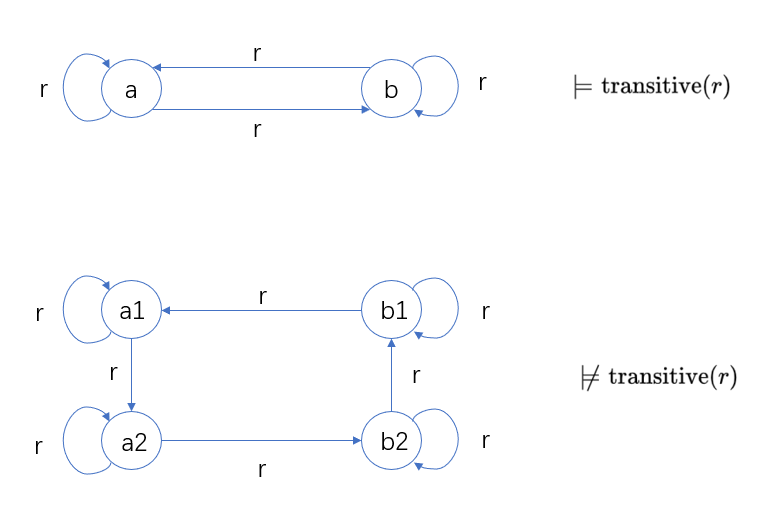
\includegraphics[width=0.8\textwidth]{11_2.png}\\
			\label{fig:roc}
			\end{figure}
        As shown in the picture above, $\mathcal{I}_1 \sim \mathcal{I}_2$, so there is not a \\
        $\mathcal{ALC}$-Concept could distinguish the two interpretations, but $\mathcal{S}$-Concept $transitive(r)$ can distinguish $\mathcal{I}_1$ and $\mathcal{I}_2$. \\
        Therefore $\mathcal{S}$ is more expressive than $\mathcal{ALC}$.
    \end{enumerate}
    \paragraph{Question 12. Bisimulation invariance}~{}
    \\
    
    \begin{enumerate}
        \item[(1)]
        Definition of $\mathcal{ALCN}$-bisimulation: \\
        let $\mathcal{I}_1$ and $\mathcal{I}_2$ be Interpretations. The relation $\rho \subset \Delta^{\mathcal{I}_1}\times \Delta^{\mathcal{I}_2}$ is a bisimulation between $\mathcal{I}_1$ and $\mathcal{I}_2$ iff: \\
        a. $d_1 \rho d_2 \text{ implies } d_1 \in A^{\mathcal{I}_1} \text{ iff } d_2 \in A^{\mathcal{I}_2} \text{ for all } A \in \bold{C}$ \\
        b. $d_1 \rho d_2 \text{ and } (d_1, d_1^{'}) \in r^{\mathcal{I}_1} \text{ implies the existence of } d_2^{'} \in \Delta^{\mathcal{I}_2} \text{ such that } d_1^{'} \rho d_2^{'} \text{ and } $ \\
        $(d_2, d_2^{'})\in r^{\mathcal{I}_2} \text{ for all }r \in \bold{R}$ \\
        c. $d_1 \rho d_2 \text{ and } (d_2, d_2^{'}) \in r^{\mathcal{I}_2} \text{ implies the existence of } d_a^{'} \in \Delta^{\mathcal{I}_1} \text{ such that } d_1^{'} \rho d_2^{'} \text{ and } $ \\
        $(d_1, d_1^{'})\in r^{\mathcal{I}_1} \text{ for all }r \in \bold{R}$ \\
        d. $d_1 \rho d_2 \text{ and } \text{ card} \left(\left\{d \in \Delta ^{\mathcal{I}_1} | (d_1, d) \in r^{\mathcal{I}_1}\right\}\right) = n (n \in \bold{Z})\text{ implies } $ \\
        $\text{ card} \left(\left\{d \in \Delta ^{\mathcal{I}_2} | (d_2, d) \in r^{\mathcal{I}_2}\right\}\right) = n\text{ for all } r\in \bold{R} $ \\
        e. $d_1 \rho d_2 \text{ and } \text{ card} \left(\left\{d \in \Delta ^{\mathcal{I}_2} | (d_2, d) \in r^{\mathcal{I}_2}\right\}\right) = n (n \in \bold{Z})\text{ implies } $ \\
        $\text{ card} \left(\left\{d \in \Delta ^{\mathcal{I}_1} | (d_1, d) \in r^{\mathcal{I}_1}\right\}\right) = n\text{ for all } r\in \bold{R} $ \\
        \item[(2)]
        Firstly, we need to prove the bisimulation invariance of $\mathcal{ALCQ}$.We just have to prove the case when $C = (\leq n)r.$, 
        other cases are as the same as $\mathcal{ALC}$. \\
        let: $C = (\leq n)r.$, if $d_1 \in C^{\mathcal{I}_1}$, then $\text{ card} \left(\left\{d \in \Delta ^{\mathcal{I}_1} | (d_1, d) \in r^{\mathcal{I}_1}\right\}\right) \leq n$, if 
        $(\mathcal{I}_1, d_1) \sim (\mathcal{I}_2, d_2)$, then  $\text{ card} \left(\left\{d \in \Delta ^{\mathcal{I}_1} | (d_2, d) \in r^{\mathcal{I}_1}\right\}\right) \leq n$, so $d_2 \in C^{\mathcal{I}_1}$ \\
        Secondly, we show that there exists models which $\mathcal{ALCN}$ could not distinguish but $\mathcal{ALCQ}$ could do that. \\
        \begin{figure}[h]
			\centering
			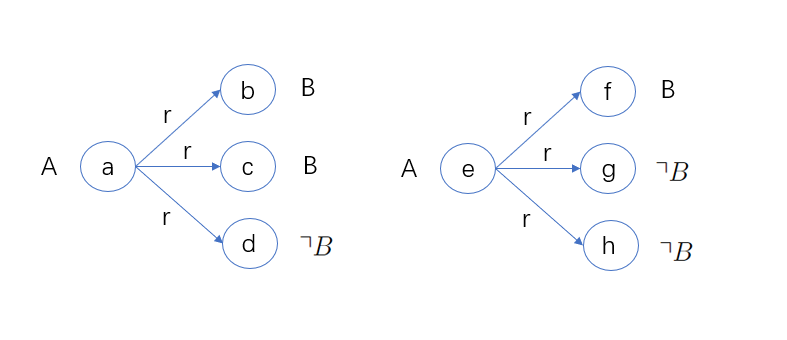
\includegraphics[width=0.8\textwidth]{12_2.png}\\
			\label{fig:roc}
			\end{figure}
        According to the def of bisimulation of $\mathcal{ALCN}$, $(\mathcal{I}_1, a) \sim (\mathcal{I}_2, e)$, so there is not a 
        $\mathcal{ALCN}$-Concept could distinguish $a$ and $e$, but $\mathcal{ALCN}$-Concept $(\leq 1)r. \urcorner B$ can distinguish $d_1$ and $e_1$. \\
        Therefore $\mathcal{ALCQ}$ is more expressive than $\mathcal{ALCN}$.
    \end{enumerate}

    \paragraph{Question 13. Make the acquaintance of Prote´ge´}~{}
    \\

    \begin{enumerate}
        \item[(1)]
        axiom count: 801; logical axiom count: 322 \\
        They are different because axiom consists of logical axioms and non-logic axioms. Logic axioms are the axioms that could be used to reasoning, while non-axioms do not have
        the function, such as declaration axioms and annotation assertions.
        \item[(2)]
        \begin{enumerate}
            \item[(1.1)]
            use nominals: Country is EquivalentTo DomainThing and ({ America, England, France, Germany, Italy })
            \item[(1.2)]
            use nogations: \\ VegetarianPizza EquivalentTo Pizza and (not (hasTopping some SeafoodTopping)) and (not (hasTopping
some MeatTopping)) \\
            NonVegetarianPizza EquivalentTo Pizza and (not VegetarianPizza) \\
            \item[(1.3)]
            declare a sub-property of an object property:\\
            hasTopping SubPropertyOf: hasIngredient \\
            isBaseOf SubPropertyOf: isIngredientOf \\
            isToppingOf SubPropertyOf: isIngredientOf \\
            hasBase SubPropertyOf: hasIngredient \\
            \item[(1.4)]
            declare an inverse property: \\
            hasBase InverseOf isBaseOf \\
            hasTopping InverseOf isToppingOf \\
            hasIngredient InverseOf isIngredientOf \\
        \end{enumerate} 
        \item[(3)]
        \begin{figure}[h]
			\centering
			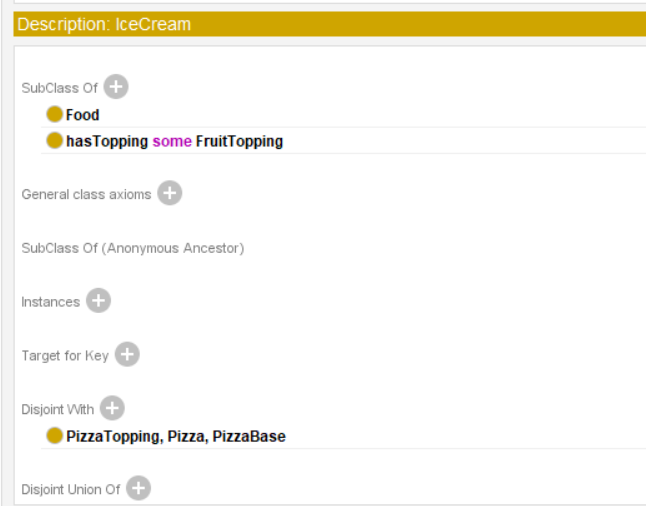
\includegraphics[width=0.8\textwidth]{13_3.png}\\
			\label{fig:roc}
			\end{figure}
        Because IceCream is equivalent to Nothing. IceCream has a restriction "SubClassOf hasTopping some FruitTopping", but hasTopping
        has a domain of Pizza, which is disjoint with IceCream(we can see this in the picture), So there's a contradiction.
        \item[(4)]
        class ::: superclass \\
        CajunSpiceTopping: SpicyTopping. \\
        SloppyGiuseppe: CheesyPizza, InterestingPizza, MeatyPizza, SpicyPizza, SpicyPizzaEquivalent. \\
        \item[(5)]
        \begin{figure}[h]
			\centering
			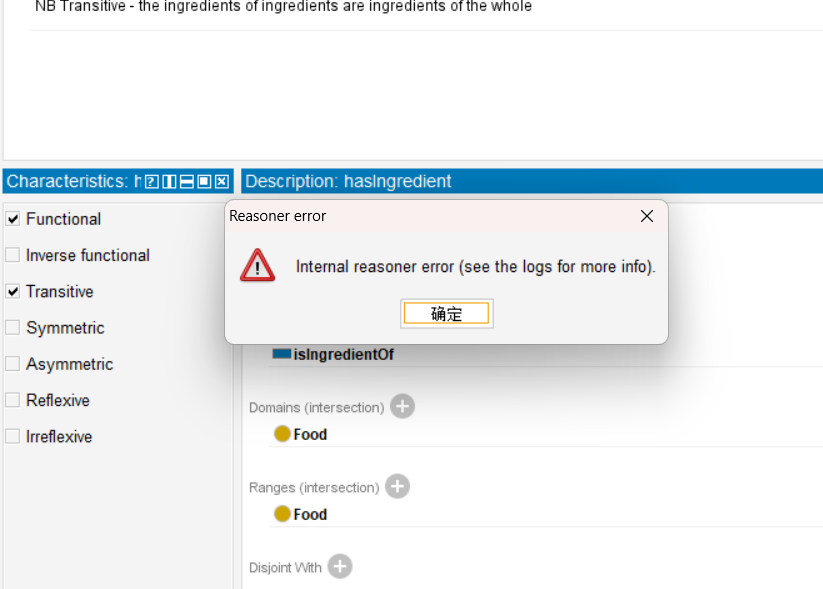
\includegraphics[width=0.8\textwidth]{13_5.png}\\
			\label{fig:roc}
			\end{figure}
        It will throw a warning(as the picture). Because there are some food have various ingredient, so the object property "hasIngredient" is not a function.
    \end{enumerate}

    \newpage 
    \paragraph{Question 14. Develop your first ontology with Prote´ge´}~{}
    \\

    \begin{figure}[h]
        \centering
        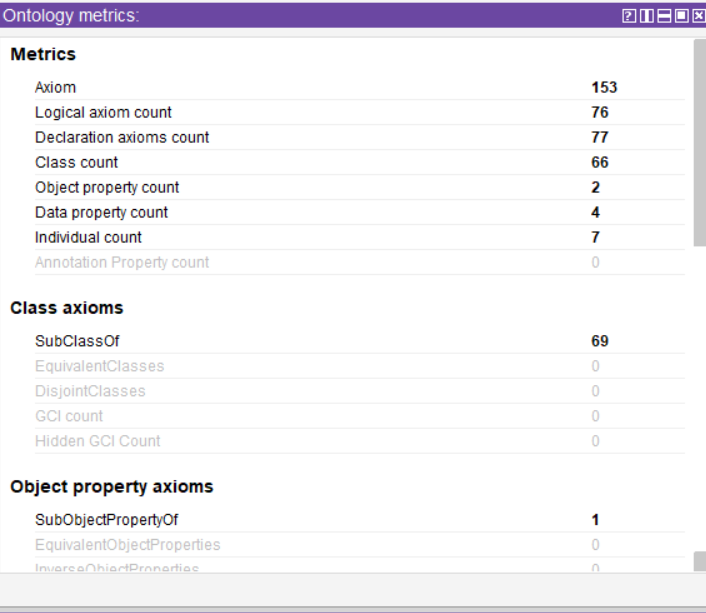
\includegraphics[width=0.8\textwidth]{14_1.png}\\
        \caption{Ontology metrics}
        \label{fig:roc}
        \end{figure}
    \begin{figure}[h]
        \centering
        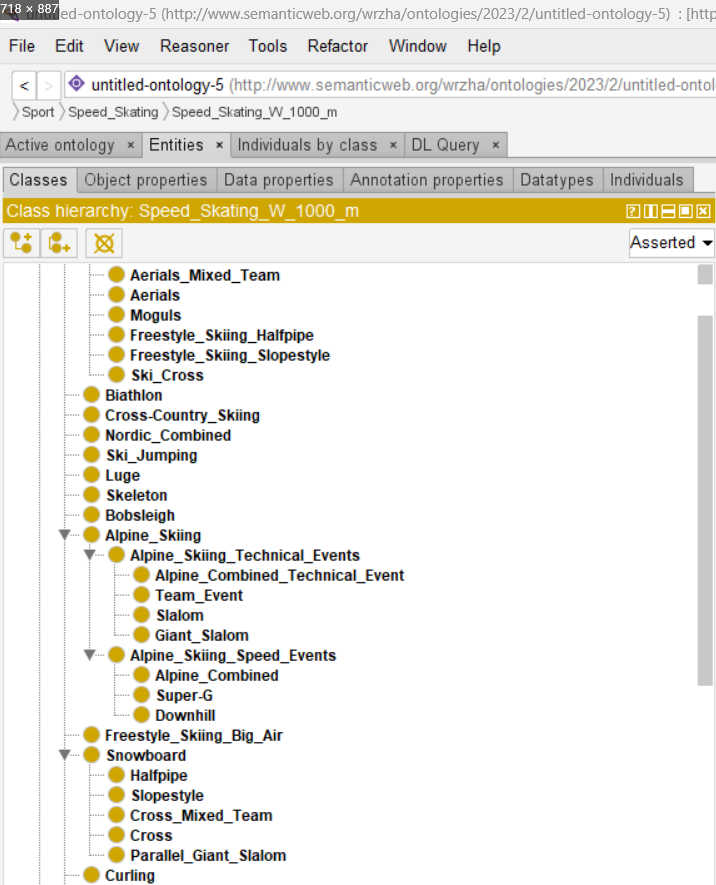
\includegraphics[width=0.8\textwidth]{14_2.png}\\
        \caption{ Hierarchy of sports items}
        \label{fig:roc}
        \end{figure}
        \begin{figure}[h]
            \centering
            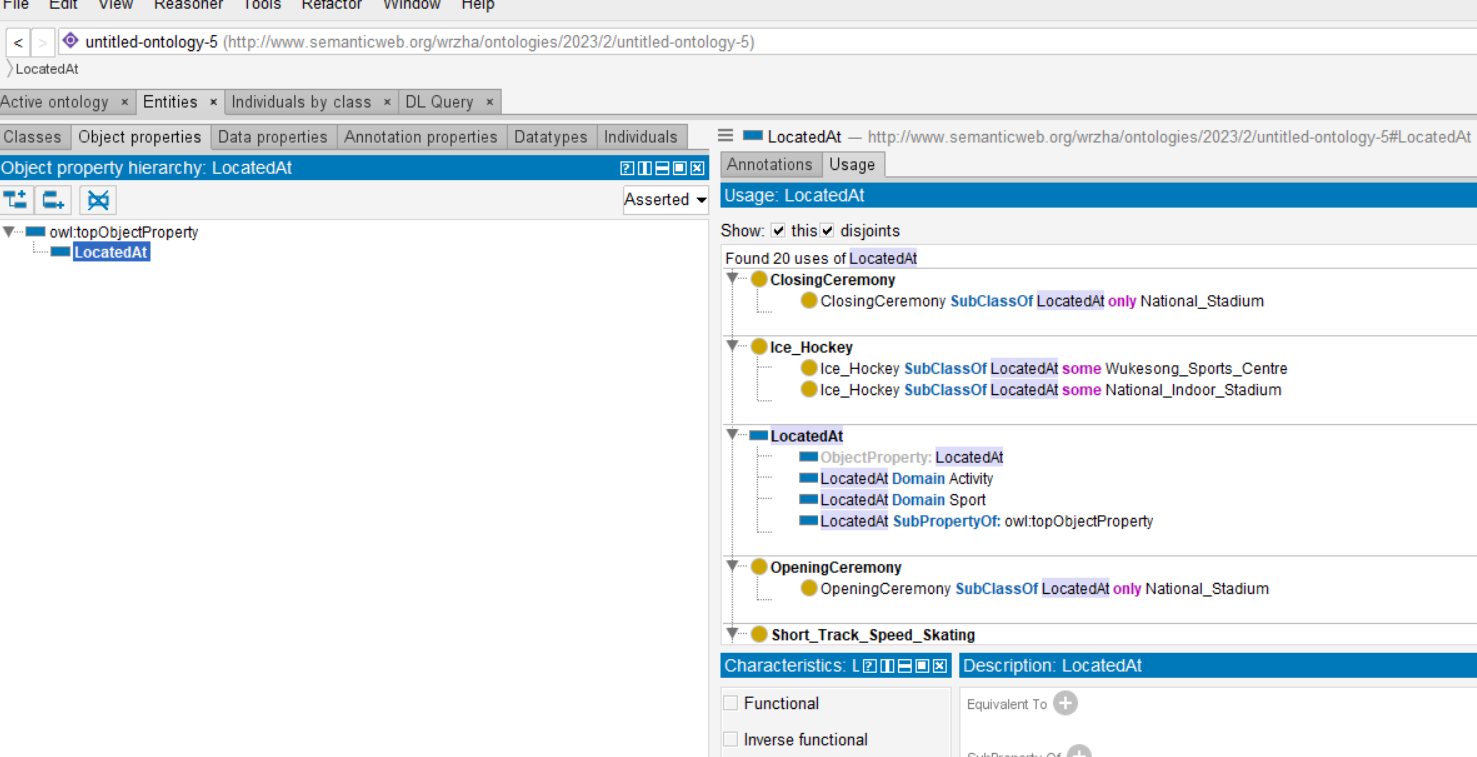
\includegraphics[width=0.8\textwidth]{14_3.png}\\
            \caption{Object properties: LocatedAt}
            \label{fig:roc}
            \end{figure}
            \begin{figure}[h]
                \centering
                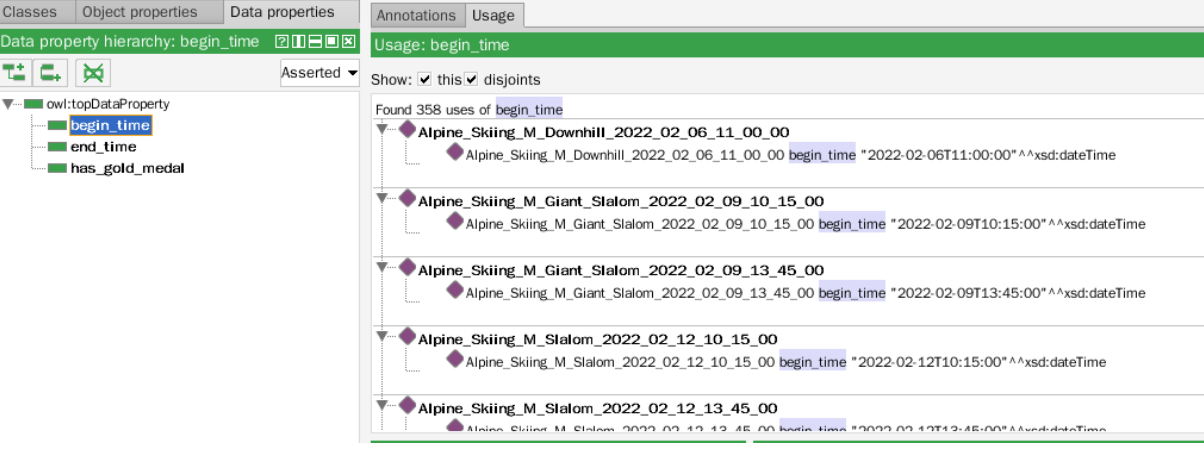
\includegraphics[width=0.8\textwidth]{14_4.png}\\
                \caption{ Data properties: begin, end time}
                \label{fig:roc}
                \end{figure}
                \begin{figure}[h]
                    \centering
                    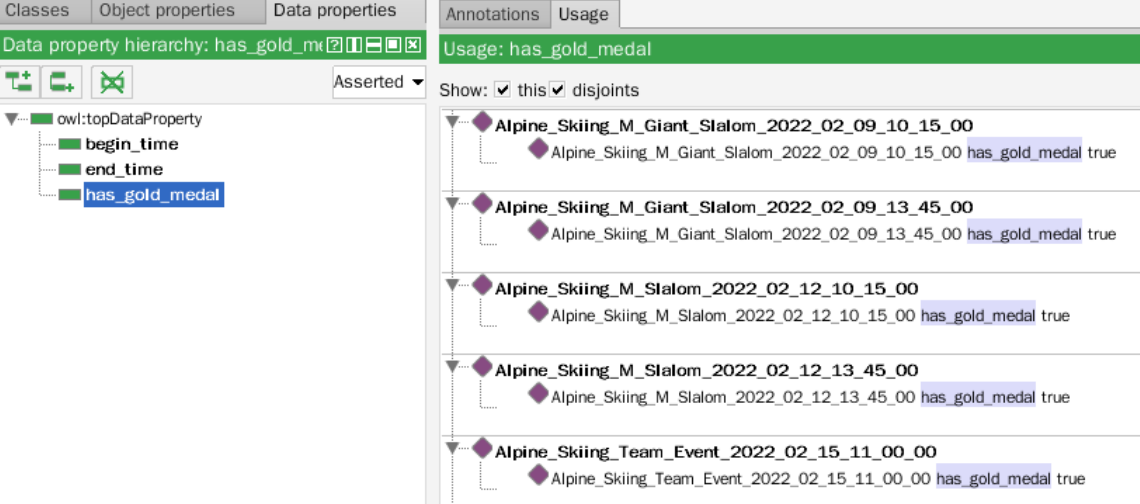
\includegraphics[width=0.8\textwidth]{14_5.png}\\
                    \caption{ Data properties: gold medals}
                    \label{fig:roc}
                    \end{figure}
        As the picture show, I built a hierarchy of sports, activity and place(Figure 2), 
        I built a object properties to represent the stadium of a sport(Figure 3), I built two
        data properties to represent the begin time and end time of each sport(Figure 4), I built a
        data property to represent whether a game produces a gold medal(Figure 5).
\end{document}
